\section{Finite state automata}

\begin{definition}
    A \emph{finite state automaton} (FSA) consists of the following three elements: 
    \begin{enumerate}
        \item The input tape, which contains the input string $x \in \Sigma^{*}$. 
        \item The control unit and its finite memory, which contains the state table.  
        \item The input head, initially positioned at the start marker of string $x$, which is shifted to the right at every move, as far as it reaches the end-marker of string $x$ or an error happens.
    \end{enumerate}
\end{definition}

After reading an input character, the automaton updates the current state of the control unit. 

After scanning the input string $x$, the automaton recognizes string $x$ or rejects it, depending on the current state.

\begin{definition}
    The \emph{state-transition graph} is a directed graph that represents the automaton and consists of the following elements: 
    \begin{itemize}
        \item Nodes: represent the states of the control unit. 
        \item Arcs: represent the moves of the automaton. 
    \end{itemize}
\end{definition}

Each arc is labeled by an input symbol, and it represents the move enabled when the current state matches the source state of the arc and the current input symbol matches the arc label. 
The state-transition graph has a unique initial state, but it may have none, one or more final states. 

The graph can be represented in the form of an incidence matrix. 
Each matrix entry is indexed by the current state and by the input symbol, and contains the next state.
Such an incidence matrix is often called state table. 
It is possible to use a syntax diagram, that is the dual of the state-transition graph (nodes are transformed into vertices and the other way around).
\begin{example}
    Given the language over the alphabet $\Sigma=\delta \cup \{0,\cdot\}$, where $\delta=\{1,2,3,4,5,6,7,8,9\}$ can be used to generate the decimal numbers. 
    The regular expression to do so is as follows: 
    \[e=\left( 0 \cup \delta (0 \cup \delta)^{*} \right) \cdot (0 \cup \delta)^{+}\]
    The corresponding state-transition graph is as follows: 
    \begin{figure}[H]
        \centering
        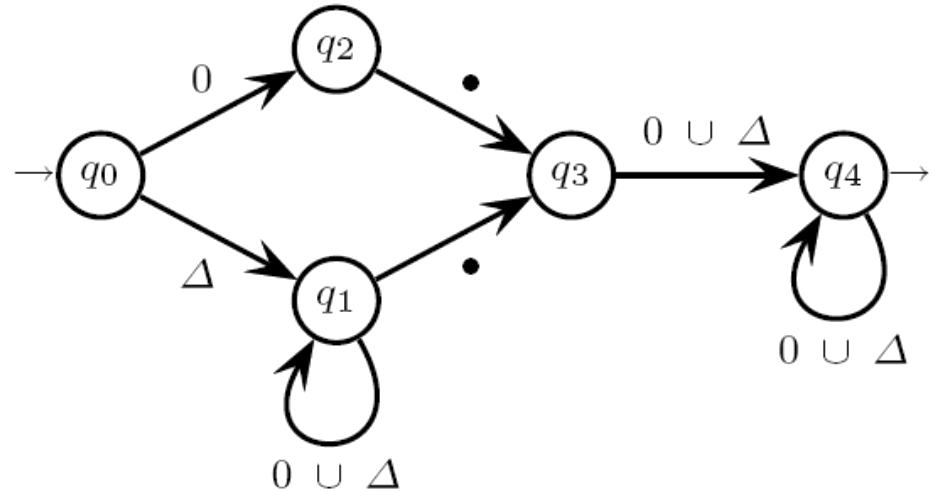
\includegraphics[width=0.5\linewidth]{images/fsa1.png}
    \end{figure}
    And the state-transition table is: 
    \begin{table}[H]
        \centering
        \begin{tabular}{|c|ccccc|}
        \hline
        \textbf{Current state} & \multicolumn{5}{c|}{\textbf{Current character}}\\ \cline {2-6}
                               & 0      & 1      & $\dots$  & 9      & $\cdot$  \\ \hline
        $\rightarrow q_0$      & $q_2$  & $q_1$  & $\dots$  & $q_1$  & -        \\
        $q_1$                  & $q_1$  & $q_1$  & $\dots$  & $q_1$  & $q_3$    \\
        $q_2$                  & -      & -      & $\dots$  & -      & $q_3$    \\
        $q_3$                  & $q_4$  & $q_4$  & $\dots$  & $q_4$  & -        \\
        $q_4 \rightarrow$      & $q_4$  & $q_4$  & $\dots$  & $q_4$  & -        \\ \hline
        \end{tabular}
    \end{table}
    The syntax diagram is: 
    \begin{figure}[H]
        \centering
        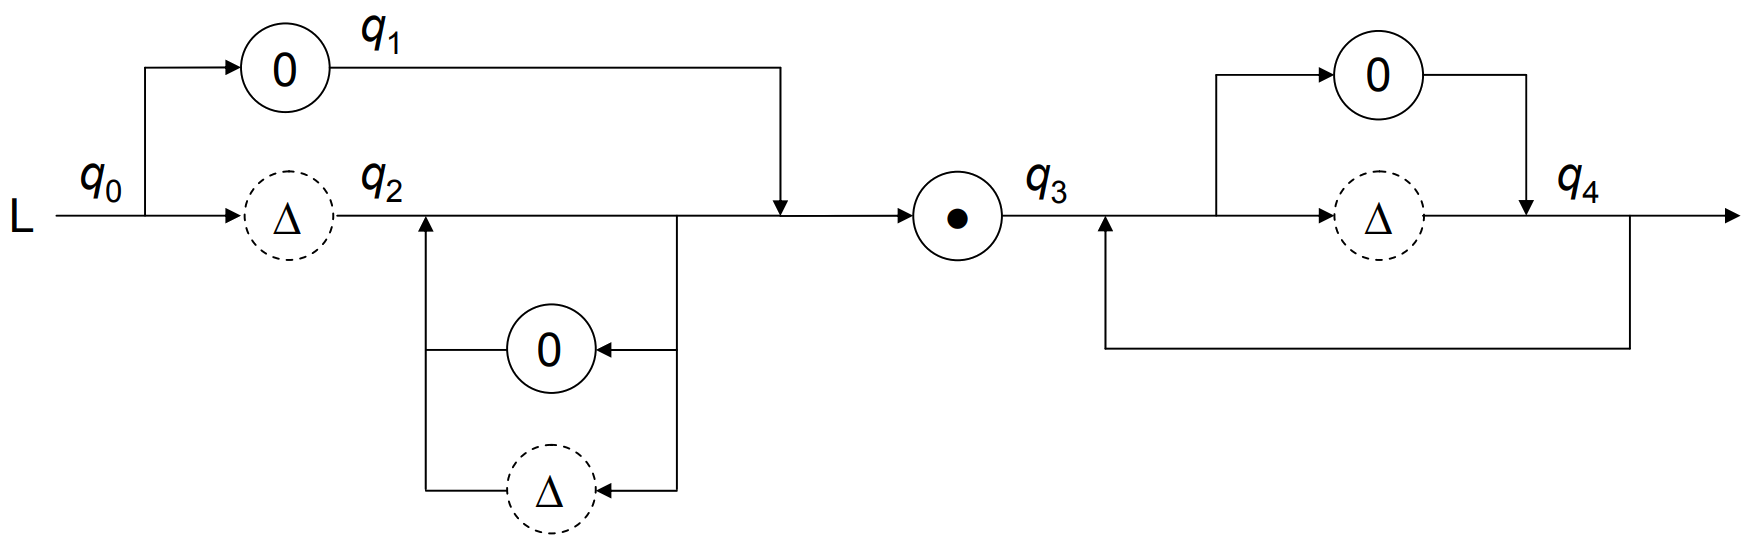
\includegraphics[width=0.75\linewidth]{images/fsa2.png}
    \end{figure}
\end{example}